\documentclass{llncs}
\usepackage{graphicx}
\usepackage{booktabs} % allows \toprule and other table formatting utilities
\usepackage{multirow} % merge cells vertically
%\usepackage{lscape} % Landscape orientation (used for tables)
\usepackage{colortbl} % Allows for alternate coloring the table
\usepackage[table]{xcolor} % U.a. allows for defining colors in HTML models
\usepackage{rotating} % Landscape orientation (used for tables)
\usepackage{color} % Only required for the TODO macro.

%\usepackage{natbib}
%

\usepackage[pdfborder={0 0 0}]{hyperref} % links, but no colored boxes

\hypersetup{breaklinks=true,
pagecolor=white,
colorlinks=false}
\urlstyle{rm} %so it doesn�t use a typewriter font for url�s.

% Allow line breaks in texttt
\newcommand{\origttfamily}{}% sollte noch nicht definiert sein!
\let\origttfamily=\ttfamily % alte Definition von \ttfamily sichern
\renewcommand{\ttfamily}{\origttfamily \hyphenchar\font=`\-}



%%%%%%%%%%%%%%%%%%%%%%%%%%%%%%%%%%%%%%%%%%%%%%
% Some macros
%%%%%%%%%%%%%%%%%%%%%%%%%%%%%%%%%%%%%%%%%%%%%%
%%%%%%%%%%%%%%%%%%%%%%%%%%%%%%%%%%%%%%%%%%%%%%
\def\plus{\textsuperscript{+}}
\newcommand{\TODO}[1]{\textcolor{red}{\textbf{#1}}}

% B
\newcommand{\BiochemicalReaction}{\texttt{Bio\-chemical\-Reaction}}
\newcommand{\BiochemicalReactions}{\texttt{Bio\-chemical\-Reaction}s}

% C
\newcommand{\Catalysis}{\texttt{Cata\-lysis}}
\newcommand{\ComplexAssembly}{\texttt{Complex\-Assembly}}
\newcommand{\Conversion}{\texttt{Conversion}}
\newcommand{\control}{\texttt{control}}
\newcommand{\Control}{\texttt{Control}}
\newcommand{\Controller}{\texttt{Controller}}
\newcommand{\Controllers}{\texttt{Controller}s}
\newcommand{\Controlled}{\texttt{Controlled}}
\newcommand{\conversion}{\texttt{conversion}}
\newcommand{\Complex}{\texttt{Complex}}

% I
\newcommand{\Interaction}{\texttt{Inter\-action}}
\newcommand{\InteractionVocabulary}{\texttt{Inter\-action\-Vo\-ca\-bu\-la\-ry}}

% M
\newcommand{\model}{\texttt{model}}
\newcommand{\Modulation}{\texttt{Modulation}}
\newcommand{\MolecularInteraction}{\texttt{Mo\-le\-cu\-lar\-In\-ter\-ac\-tion}}
\newcommand{\ModifierSpeciesReference}{\texttt{Mo\-di\-fier\-Species\-Reference}}


% P
%\newcommand{\PhysicalEntity}{\texttt{Physical\-Entity}}
\newcommand{\physicalInteraction}{\texttt{physical\-Inter\-action}}

% Q
\newcommand{\qualitativeModel}{\texttt{qualitative\-Model}}
%\newcommand{\quantitativeModel}{\texttt{quantitative\-Model}}
\newcommand{\qualitativeSpecies}{\texttt{qualitative\-Species}}

% R
\newcommand{\reaction}{\texttt{re\-ac\-tion}}
\newcommand{\reactions}{\texttt{re\-ac\-tion}s}

% S
\newcommand{\species}{\texttt{species}}
\newcommand{\SmallMolecules}{\texttt{Small\-Molecule}s}


% T
\newcommand{\TemplateReactionRegulation}{\texttt{Template\-Reaction\-Regulation}}
\newcommand{\TemplateReaction}{\texttt{Template\-Reaction}}
\newcommand{\transition}{\texttt{transition}}
\newcommand{\transitions}{\texttt{transition}s}
\newcommand{\Transport}{\texttt{Transport}}
\newcommand{\TransportWithBiochemicalReaction}{\texttt{Transport\-With\-Biochemical\-Reaction}}

%%%%%%%%%%%%%%%%%%%%%%%%%%%%%%%%%%%%%%%%%%%%%%
%%%%%%%%%%%%%%%%%%%%%%%%%%%%%%%%%%%%%%%%%%%%%%
\hyphenation{
bal-ance
con-ver-ter
KEGG-con-ver-ter
}



%%% PAGE NUMBERS (only for corrections) %%%
%\usepackage{scrpage2}
%\pagestyle{scrheadings}
%%%%%%%%%%%%%%%%%%%%%%%%%%%%%%%%%%%%%%%%%%%%%%

\begin{document}

\title{Precise generation of systems biology models from KEGG pathways}
%\textcolor{red}{\small{ALTERNATIVE: Preparing KEGG pathway models for various applications}}
\titlerunning{KEGG pathways to systems biology models}

\author{Clemens Wrzodek\inst{1} \and Finja B\"uchel\inst{1} \and Andreas Dr\"ager\inst{1} \and Manuel Ruff\inst{1} \and Andreas Zell\inst{1}}
\authorrunning{Wrzodek \emph{et al.}}

\institute{Center for Bioinformatics Tuebingen (ZBIT), University of Tuebingen, T\"ubingen, Germany}

\maketitle


\begin{abstract}
The KEGG PATHWAY database provides a plethora of pathways for a diversity of organisms.
All pathway components are directly linked to other KEGG databases, such as KEGG COMPOUND, KEGG REACTION, etc.
%Subsequently, the pathways can be used as foundations for initial structural modeling approaches, which is further eased by providing an enormous amount of information from other cross-linked KEGG databases.
Therefore, the pathways can be extended with an enormous amount of information and provide a foundation for initial structural modeling approaches.
%
But the KGML-formatted KEGG pathways are primarily intended for visualization purposes and thus, a direct conversion into systems biology models would produce incomplete and erroneous models.

Here, we present a method for preprocessing and precisely converting KEGG pathways into initial structural models in the standardized community pathway formats SBML (Levels 2 and 3) and BioPAX (Levels 2 and 3).
This method involves fixing invalid or incomplete KGML content, atom balance check of reactions, and augmenting the pathway content with various information, such as cross-references to Entrez Gene, OMIM, UniProt ChEBI, etc.
Furthermore, we show that the conversion from KEGG to BioPAX does not involve a loss of information, whilst lossless translations to SBML can only be performed using SBML Level~3, including its recently proposed qualitative models and groups extension packages.

%\rule{\textwidth}{0.5mm}
%\TODO{Alternativer (schlechterer?) abstract:}
%
%Using KEGG pathways as models is a long-lasting desire in systems biology. Many of those pathways can be used as foundations for initial structural modeling approaches. But the KGML-formatted KEGG pathways are primarily thought for visualization and thus, incomplete and erroneous when directly converted to systems biology models. Many things have to be considered and many processing steps are required, prior to the conversion into standardized community pathway formats.
%
%We here propose methods to convert KEGG pathways to initial structural models in SBML (level 2 and 3) and BioPAX (level 2 and 3). Further, multiple aspects of KEGG and KGML files are described, together with their implications on the resulting models. We show that correct translations to SBML without loss of information can only be done with SBML level~3, using the recently proposed qualitative models (qual) and groups extensions.



% Es ist w�nschenswert KEGG pathways als modelle in der systembiologie zu verwenden.
% Hierbei gibt es viele schwierigkeiten, [andere (konnten) diese gar nicht �berwinden]
%

%problem statement:
%      what problem are you going to solve?
%
%motivation/relevance:
%      why is it important to solve this problem?
%
%approach/method:
%      how did you go about solving the problem?
%
%results:
%      what is your solution to the problem?
%
%conclusions:
%      what are the implications of your solution?
\end{abstract}

\section{Introduction}
%Opening statement
%    Problem: what problem are you going to solve?
%    Relevance: why is it important to solve this problem?
%
%Literature review:
%    Summarize the current state of knowledge in the area of
%              investigation
%    What previous research has been done on the problem?
%    Mark the gap in the current state of knowledge:
%    What piece of knowledge is still lacking in the area of
%              investigation?
%
%Brief overview of your own study:
%    Approach/method: how did you go about filling this gap?
%    Results: what did you find out?
%    Conclusion: what do these results mean (why are these
%               results significant?

% 1. KEGG ist toll weil
% 2. Modelling
% 3. ...und man k�nnte tolle Sachen machen wenn man tolle Modelle h�tte.
% 4. Deshalb gibt es Converter
The KEGG PATHWAY database provides a valuable resource for initial modeling approaches of specific biological networks \cite{Kanehisa2000,KEGG}. The database contains pathway maps for a multitude of different organisms and most provided information is cross-linked with other KEGG databases. For many years, this database is one of the most important sources for building initial structural models of various pathways \cite{Bauer-Mehren2009,Oberhardt2009}. All pathway information is stored in KGML formatted XML-files, which are barely supported by other applications. In systems biology, two wide-spread formats for modeling and exchanging pathways are the SBML and BioPAX formats \cite{Finney2003,Demir2010}. These formats can be used with graphical modeling applications (e.g., CellDesigner \cite{Funahashi2008} or Cytoscape \cite{Cytoscape}), complemented with rate laws (e.g., SBMLsqueezer \cite{SBMLSqueezer}), used for flux balance analysis (e.g., FASIMU \cite{Fasimu}), etc. Therefore, converters exist that perform mostly basic conversions from KGML to those formats \cite{KEGGconverter,KEGG2SBML,SuBliMinaL}. The drawback of many of those conversions is, that even for creating initial models a basic translation of a KGML document to, e.g., an SBML document is not sufficient.

% 5. Wo ist das Problem mit den bisherigen Convertern?
The KGML documents provided by KEGG are mainly for graphical representations of pathways and consist of entries (which correspond to nodes in a pathway map), relations (which correspond to edges in a pathway map) and reactions. Those Reactions are primarily contained in metabolic pathway maps and consist of substrates, products and information about reversibility of the reaction. Given this information, it seems straightforward to derive an algorithm for viable metabolic models. But a closer look on the actual maps shows that even those reactions are mainly for visualization and not for modeling or simulation purposes. Reactions are sometimes being ``bundled", e.g., one reaction instance is built and multiple reaction identifiers, that point to different reactions, are assigned. There are often missing reactants for reactions, stoichiometric information is omitted and also the list of enzymes, catalyzing a reaction, is not necessarily entirely contained in the KGML document. Similar difficulties arise for the entries in a KGML document.
For the sake of a high-quality graphical representation of the pathway, entries or other elements are sometimes duplicated in the KGML file. When interpreting the information content of those files, duplications must be taken into account.
%
%Some pathways contain duplicate entries, which make sense for nice graphical representations but not for modeling and simulation.
%
%Furthermore, one entry might consist of multiple proteins/ genes, etc. which are grouped together for some reason.
Furthermore, a KGML document may contain references to entries, which are not physically present in the actual organism and the KGML specification even allows entries to be reactions.
All those exemplary mentioned problems show that simple one-to-one translations of KEGG pathway maps are not sufficient to build reliable and useful models.

% 6. Wie sind besser und l�sen alles.
To overcome all those drawbacks we deeply investigated the KGML documents, as well as the content of all cross-linked KEGG databases, and developed strategies for building useful initial models in SBML and BioPAX. Besides automatically fixing many of the mentioned issues, we heavily annotate and augment all provided information to ease further model building and usage of those translated pathway maps. This ranges from adding simple database cross-references (e.g., to UniProt or Entrez Gene) over annotation of chemical formulas and molecular weight of small molecules, to an automated atom balance check of all reactions. All those strategies are now included in the second release of the KEGGtranslator application \cite{Wrzodek2011} and described in detail in the following desctions.



% 1. KEGG ist toll weil
% 2. Wo ist das Problem (beschreibt grafische Zusammenh�nge)
% Verschiedene Formate f�r versch. Sachen, nicht verlustfrei m�glich
% Man braucht (korrekte) Gleichungen, am besten noch chemische formeln, molekular gewicht, etc.
% f�r graphen malen braucht man gr��e, position, farbe, noch entrez gene, uniprot (und kanten)
% Inhalt ist f�r grafik, Reaktionen da fehlt einiges, sowie annotationen, etc.
% Relationen zu qual



\section{Preparation of pathway models from the KEGG database}

Several subsequent steps are involved in the creation of initial models from KEGG pathways. All of these steps are described in detail in the following sections and depicted graphically in Figure~\ref{fig:conversionScheme}

\subsection{The KEGG Markup Language (KGML)}
KEGG uses the KGML format to encode its pathways \cite{KGML}. For each pathway, a generic reference pathway is created that is derived for a plethora of different organisms. All nodes in those pathways correspond to proteins, small molecules, other referenced pathways, etc. and are encoded as entries in KGML. These entries have a type attribute that further specifies its nature. Additionally, they may have a graphics attribute that is essential for pathway visualizations. Entries corresponding to groups contain components that are reference their contained entries.

Besides entries, KGML specifies reactions, which contain substrates and products that are essentially references to the corresponding entries. The only additional information that is given for reactions is a type attribute, that is either ``reversible" or ``irreversible". Moreover, KEGG specifies so called ``relations" which are primarily important for pathway visualization. Relations contain network connections between two entries, such as ``A phosphorylates B", or ``A inhibits B" but they do not provide sufficient information for conversions to biochemical reactions.


% Among others, these entries have a type-attribute, that further specifies the object, described by this pathway, and a reaction attribute, which usually specifies one or more reactions that are catalyzed by this entry. If this entry is a group, consisting of several other entries that form a complex, the components are also annotated on this entry.

% TODO: Sehr wichtig: Wo bekommt man ueberhaupt die KGML dateien her?

% 1. Generell erkl�ren, dass fast alles per optionen kontrolliert werden kann.
% 2. KGML k�nnen "hier" (erkl�ren) heruntergeladen werden. Oder from within the application.


% 1. KeggTools.removePathwayEntries(p);
% 2. autocompleteReactions
% 2.1 split reactions, one per identifier
% 2.2 f�r jede reaktion noch fehlenden reaktanten suchen,
% 2.2.1 Ist reaktion reversibel? (Info Aus API holen, grade bei gesplitteten reaktionen manchmal fehlerhaft), wenn nein, in welcher richtung liegt sie vor
% 2.2.2 Haben wir synonyme? ("Same as" von jeder komponente aus api holen und hinterlegen)
% 2.2.3 fehlen reaktanten? => Fehlende zu KGML hinzuf�gen
% 2.2.4 fehlen enzyme? => Alle EC Nummern aus KEGG holen und abgleichen, fehlende hinzuf�gen

% 3. Stoichiometry aus den gleichungen parsen und merken
% 4. Remove white nodes (EC-Enzymes without protien instances in current organism)

% 5. Optionally: Remove orphans

\subsection{Preprocessing and fixing issues in the input KGML}

%TODO: Ersten abschnitt, einleitung spannender machen
Prior to converting the KEGG pathways to other modeling languages, several issues need to be fixed in preprocessing steps.
%KGML pathways are not complete and require preprocessing prior to conversion to other modeling languages.
Operations that are not linked to SBML or to BioPAX are performed as first step directly on the input KGML. These include operations that involve adding or removing entries from the KGML document. The actual conversion to models (SBML, BioPAX, etc.) is independent of those steps and will be performed after the preprocessing. To generate reliable models, one might want to remove links to other pathway maps from the document. These referenced pathway maps are no physical instances and thus need to be ignored for some model simulation software. However, they might be required for cross-linking pathways. Furthermore, orphans (i.e., entries that are not present in reactions or relations) might be useless for some modeling approaches and therefore may also be removed.

An important step towards building metabolic models are correct biochemical reactions. The reactions specified in the KGML require enormous preprocessing in order to reliably translate these to SBML or BioPAX. 
%
%First of all, bundled reactions need to be separated. There is no way to create balanced and correct biochemical reactions if one keeps multiple reactions that are bundled as one KGML-reaction record. Thus, one KGML-reaction is created for each actual biochemical reaction. 
%
KEGG files often contain bundled reactions. These must be disassembled into separate KGML reactions. Otherwise, it is not possible to create balanced and correct biochemical reactions if models keep multiple reactions that are bundled into one record.
Since the information provided in the KGML is limited, the KEGG API needs to be queried for further correction steps. From the KEGG API, information about reversibility of the reaction is retrieved, as well as the reaction equation, including all substrates, products, catalysts, and stoichiometric information. The reversibility is directly annotated on the reaction, the stoichiometric information has to be stored in separate classes, which are later translated to the desired output format. The equation is used to check for missing reaction participants. But simply comparing all KEGG identifiers that are present in the KGML with the reaction equation is not adequate. KEGG consists of many databases, such as COMPOUND, DRUG, GLYCAN, etc. Therefore, one compound might have multiple KEGG identifiers, e.g., one in KEGG COMPOUND and another one in KEGG DRUG. The reaction equations specify just one identifier for each participant, which is any of all available identifiers for an object. Therefore, more queries to the KEGG API are necessary in order to fetch all synonyms for all identifiers. Now, it is possible to check for missing reaction participants and eventually add those to the KGML. A similar method is required to check for missing enzymes (i.e., reaction modifiers) -- we use Enzyme Commission numbers (EC numbers) to check for missing enzymes.

%At this step, the KGML document is almost ready to be translated to a model.
One last optional preprocessing step might be performed before converting the pathways to models.
The KEGG database uses information about orthology to provide pathway maps for different organisms. Enzymes, catalyzing reactions are annotated using EC numbers, which are independent of actual organisms. In some cases, this leads to annotated enzymes or entries in the KGML, for which no physical instance in the current organism of interest is known. In other words, the entry does probably not exist in the current organism or its existence has not yet been proven. To visualize this information, KEGG changes the background color of those orthologous nodes to white. These nodes should also be removed in order to obtain organism-specific models.

\subsection{Atom balance of reactions}

After the described preprocessing step, the KGML document contains unbundled and complete reactions, for which the equation and stoichiometry has been annotated. Using the KEGG API, the chemical formula of each compound, participating in a reaction can be fetched. By using this information together with the stoichiometry, it is possible to count and compare all atoms on the substrate and product side. We detected some simple cases in which an H\plus{} or P\plus{} was missing, but also some other cases in which multiple atoms (e.g., 2C, 3H, 1P) where missing. Automatically fixing those issues is not recommended because the real missing components are unknown.
%For example if a P\plus{} is missing, the possibilities include ATP, ADP, NADPH, etc. 
For example if a P\plus{} is missing on the substrate side, the possibilities of missing components on both sides include ATP~$\longrightarrow$~ADP, NADPH~$\longrightarrow$~NADH, and many others.
Therefore, the result of each atom check is written as comment on every reaction and researchers might have to manually fix reactions with missing atoms.


\subsection{Convert and augment the KGML document}
%%%%%%%%%%%%%%%%%%%%%%%%%%%% BEGIN FIGURE  %%%%%%%%%%%%%%%%%%%%%%%%%%%%%%%%%%%%%%%%%%%%%
\begin{figure}[p]
\centering 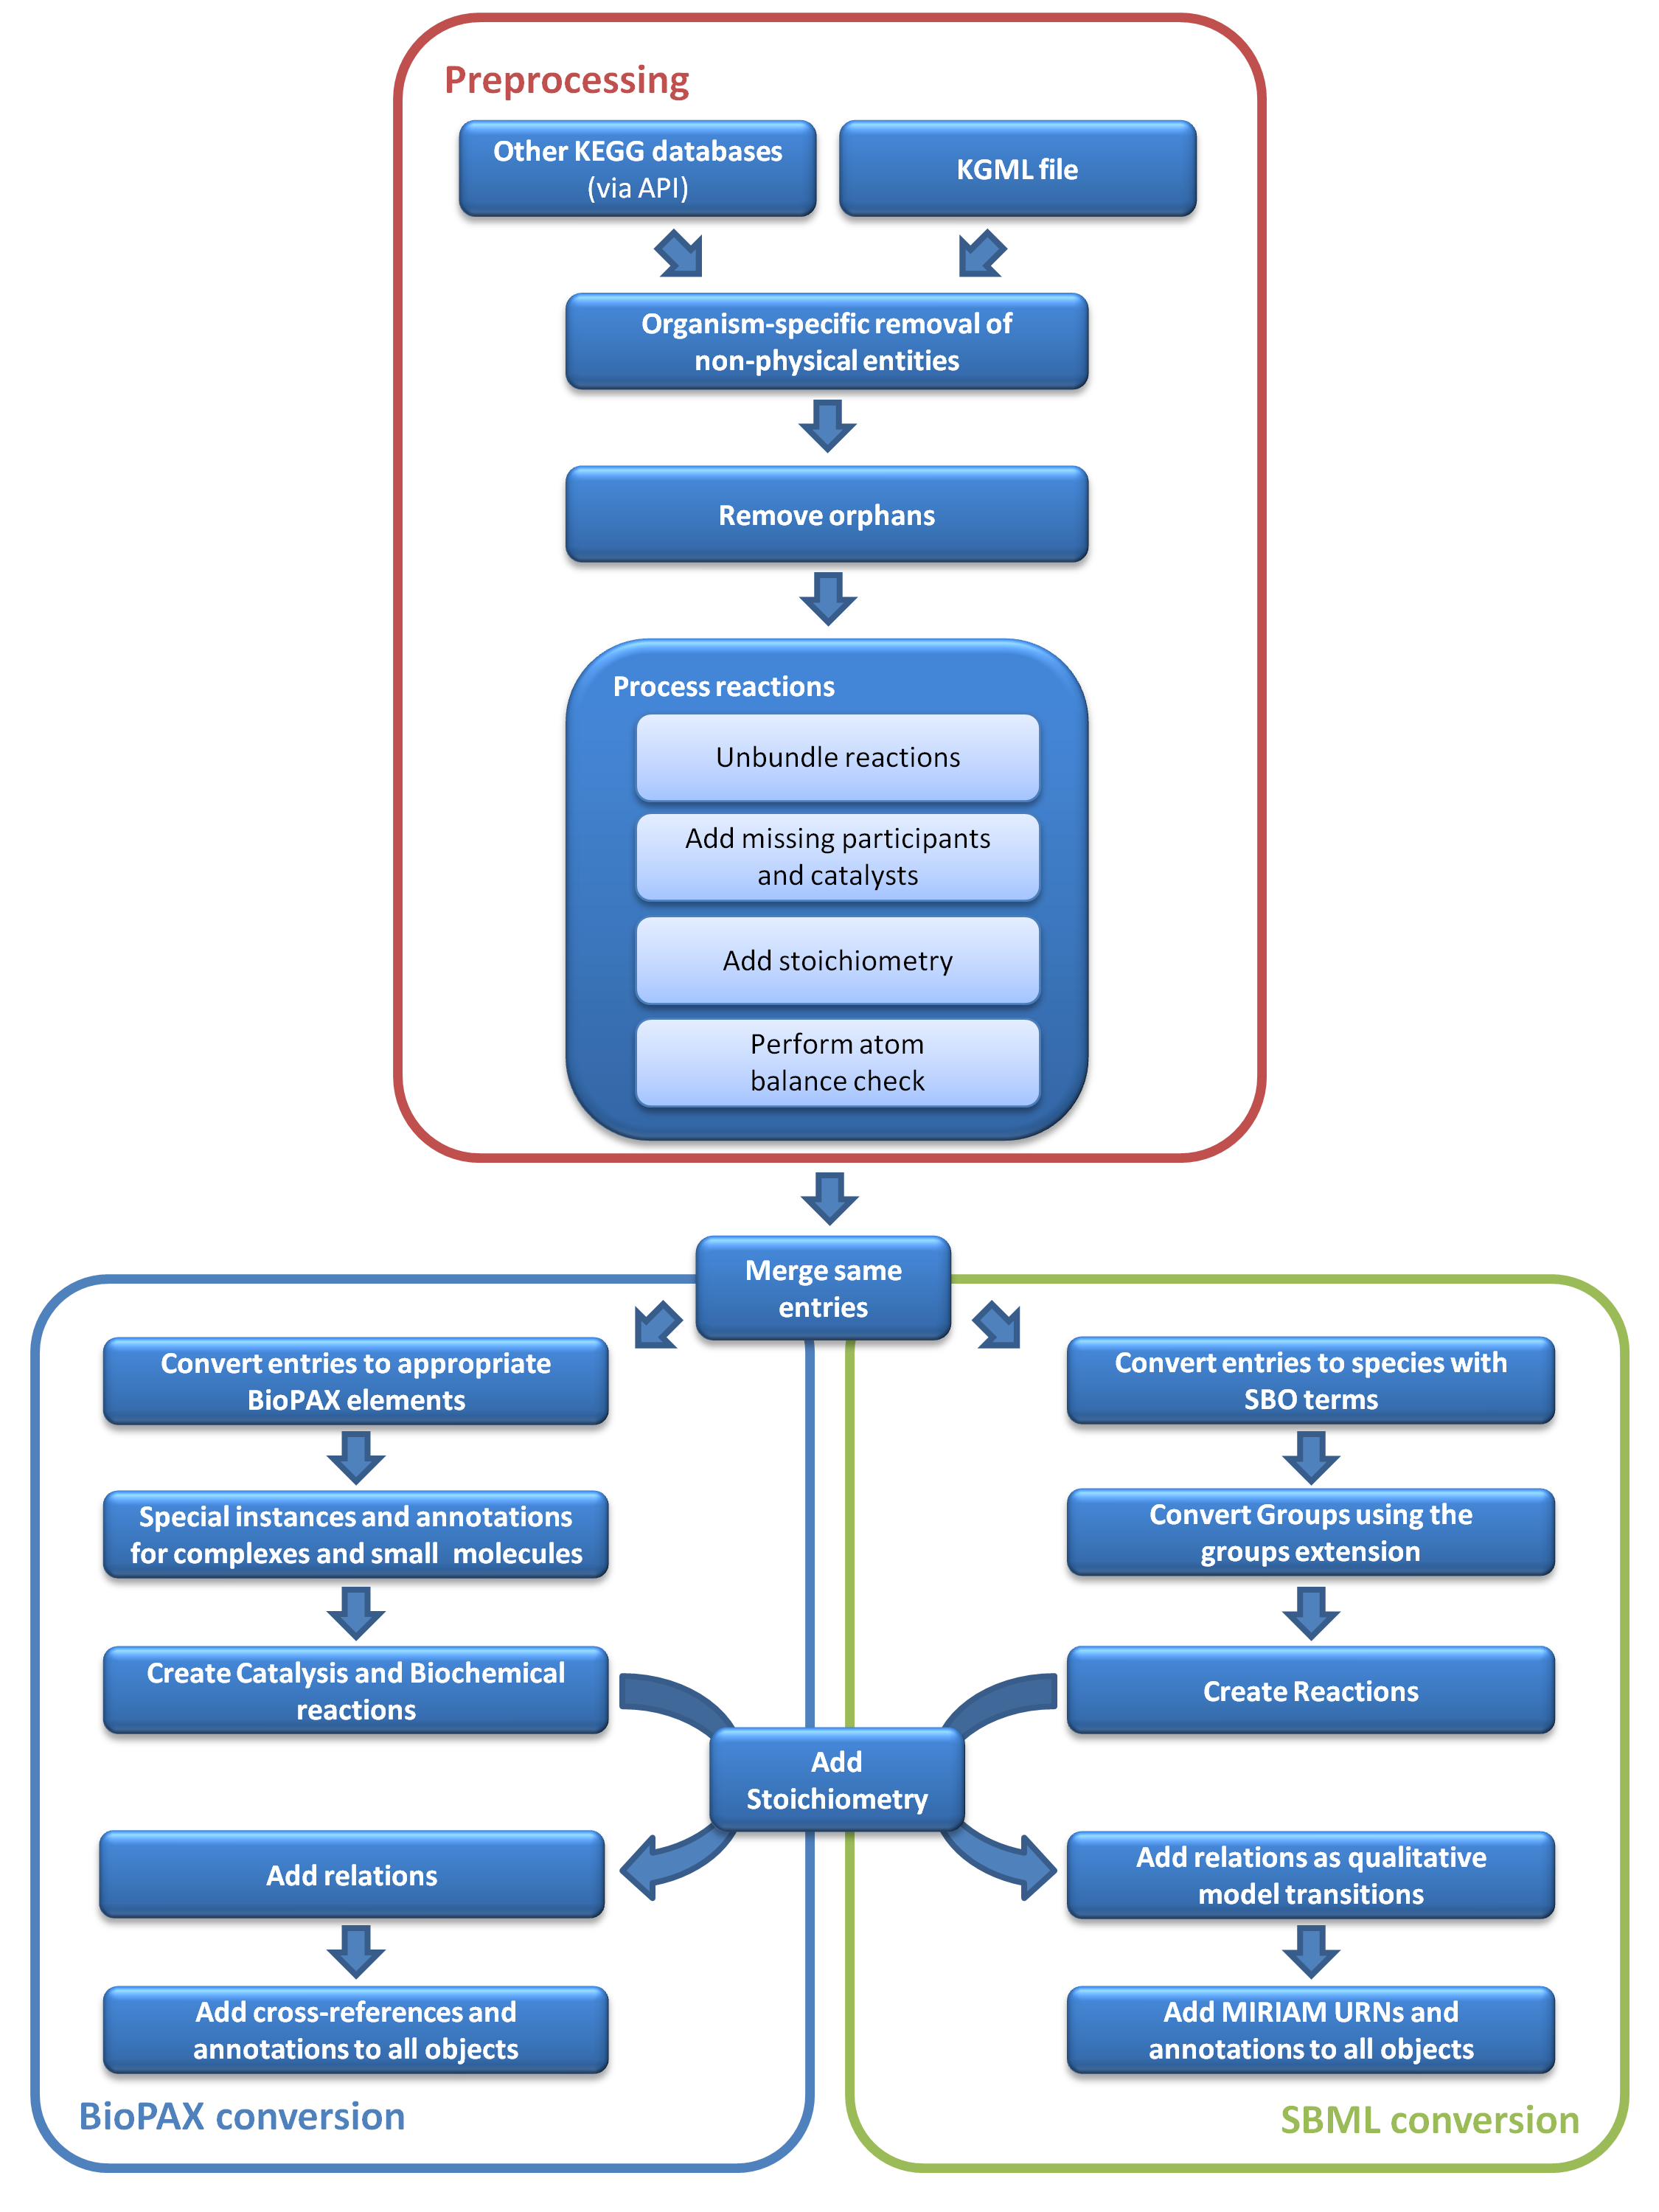
\includegraphics[width=1.0\columnwidth]{figures/Flowchart.png}
\caption{Flowchart of the conversion from KGML to BioPAX or SBML -- The figure depicts all major steps involved in the creation of initial systems biology models from KEGG pathways.
%Merging of same entries is not part of the preprocessing, because there are some applications (e.g., when using the layout extension package for SBML) for which duplicate entries need to be conserved.
}
\label{fig:conversionScheme}
\end{figure}
%%%%%%%%%%%%%%%%%%%%%%%%%%%% END FIGURE  %%%%%%%%%%%%%%%%%%%%%%%%%%%%%%%%%%%%%%%%%%%%%%%



%\definecolor{tableShade}{HTML}{F1F5FA}
%\definecolor{tableShade2}{HTML}{ECF3FE}
\definecolor{tableShade2}{gray}{0.95}
%\rowcolors{3}{white}{tableShade2}

%%%%%%%%%%%%%%%%%%%%%%%% ENTRY TABLE %%%%%%%%%%%%%%%%%%%%%%%%
\begin{table}[t]
\caption{BioPAX instances and SBO terms corresponding to KGML entry types.}
\label{tab:KGMLentries2X}
\makebox[\textwidth]{
\begin{tabular*}{1.0\textwidth}{@{\extracolsep{\fill}} llll}
\toprule
KGML entry type          & BioPAX element & SBO term & SBO name\\
\midrule
%\makebox[0pt][l]{\fboxsep0pt\colorbox{tableShade2}{\strut\hspace*{\linewidth}}}\hspace{-1mm}
%\rowcolor{tableShade2}[0cm][2cm]
compound & smallMolecule & SBO:0000247  & simple chemical \\
enzyme & protein & SBO:0000252  & polypeptide chain \\
gene & protein & SBO:0000252  & polypeptide chain \\
ortholog & protein & SBO:0000252  & polypeptide chain \\
% genes & complex & SBO:0000253  & non-covalent complex \\
group & complex & SBO:0000253  & non-covalent complex \\
map & pathway & SBO:0000552  & reference annotation \\
%reaction & interaction & SBO:0000 \\

%\multicolumn{3}{c}{\centering \textbf{BioPAX Level~3}}\\
%\midrule
%compound & SmallMolecule \\
%enzyme & Protein \\
%gene & Protein \\
%ortholog & Protein \\
%%genes & Complex \\
%group & Complex \\
%map & pathway \\
%reaction & interaction \\

\bottomrule
\end{tabular*}
}
{
This table depicts the conversion of KGML entries to BioPAX or SBML. The conversion depends on the KGML entry type attribute. For BioPAX, different class instances are initialized. Conversions to SBML always involve the creation of a \species{} with the given SBO term for each KGML entry. The KGML specification states that an entry of type ``gene" ``is a gene product (mostly a protein)" \cite{KGML}. Additionally, a ``group" ``is a complex of gene products (mostly a protein complex)" \cite{KGML}. For compatibility with previous KGML versions, please note that the deprecated type ``genes" corresponds to ``group" since KGML v0.6.1. Further, entries of type ``reaction" are not in the table, but discussed in a separate section.
}
\end{table}
%%%%%%%%%%%%%%%%%%%%%%%%%%%%%%%%%%%%%%%%%%%%%%%%%%%%%%%%%%%%%


The complete and fixed KGML document can now be used to generate models. Therefore, conversions to BioPAX, SBML, SBML-qual and several other formats are required. Typically, the model instance has to be initialized and all entries need to be added to the model. Caution needs to be taken in this step, because multiple copies of an entry might be existent in one KGML document. Usually, every graphical copy catalyzes different reactions. But for systems biology models, only one element should be created for all copies, representing a union of all physically identical entries. Furthermore, KGML specifies an entry type called ``reaction", which should not be converted to a physical entity in the resulting model.
Depending on the modeling language, either the reactions or the relations or both need to be converted to the chosen format.


Besides those conversion steps, additional steps are required in order to facilitate further modeling steps by researchers. Hence, extensive annotations and comments are added to all elements. This includes Gene Ontology terms, describing the elements and their function, as well as identifiers for a plethora of other databases for genes, proteins, interactions, structural information, small molecules, etc. In more detail, identifiers are added for Entrez Gene, OMIM, Ensembl, UniProt, ChEBI, DrugBank, Gene Ontology, HGNC, PubChem, 3DMET, NCBI Taxonomy, PDBeChem, GlycomeDB, LipidBank, EC-Numbers (enzyme nomenclature) and various KEGG databases (gene, glycan, reaction, compound, drug, pathway, orthology).
%
Besides those cross-references, other helpful human and machine-readable annotations are added, for example, official gene symbols, synonyms, human-readable descriptions, links to more resources or visualizations, and the chemical formula and molecular weight for small molecules.

This is an important step, because simulations on real data or simple experimental data visualization tools require unique identifiers to map the experimental data on the pathway structure. If models provide a simple data structure with labels, but no reference identifiers, they are hardly usable in conjunction with experimental data.


% Viele zus�tzliche infos von kegg api
% MIRIAM identifiers
% ...including GO
% Very helpful Human readable annotations such as gene symobls, descriptions, pictures for compounds, Links to Kegg db entry, etc.


\subsection{KEGG to BioPAX}

%%%%%%%%%%%%%%%%%%%%%%%%%%%% BEGIN FIGURE  %%%%%%%%%%%%%%%%%%%%%%%%%%%%%%%%%%%%%%%%%%%%%
\begin{figure}[tb]
\centering 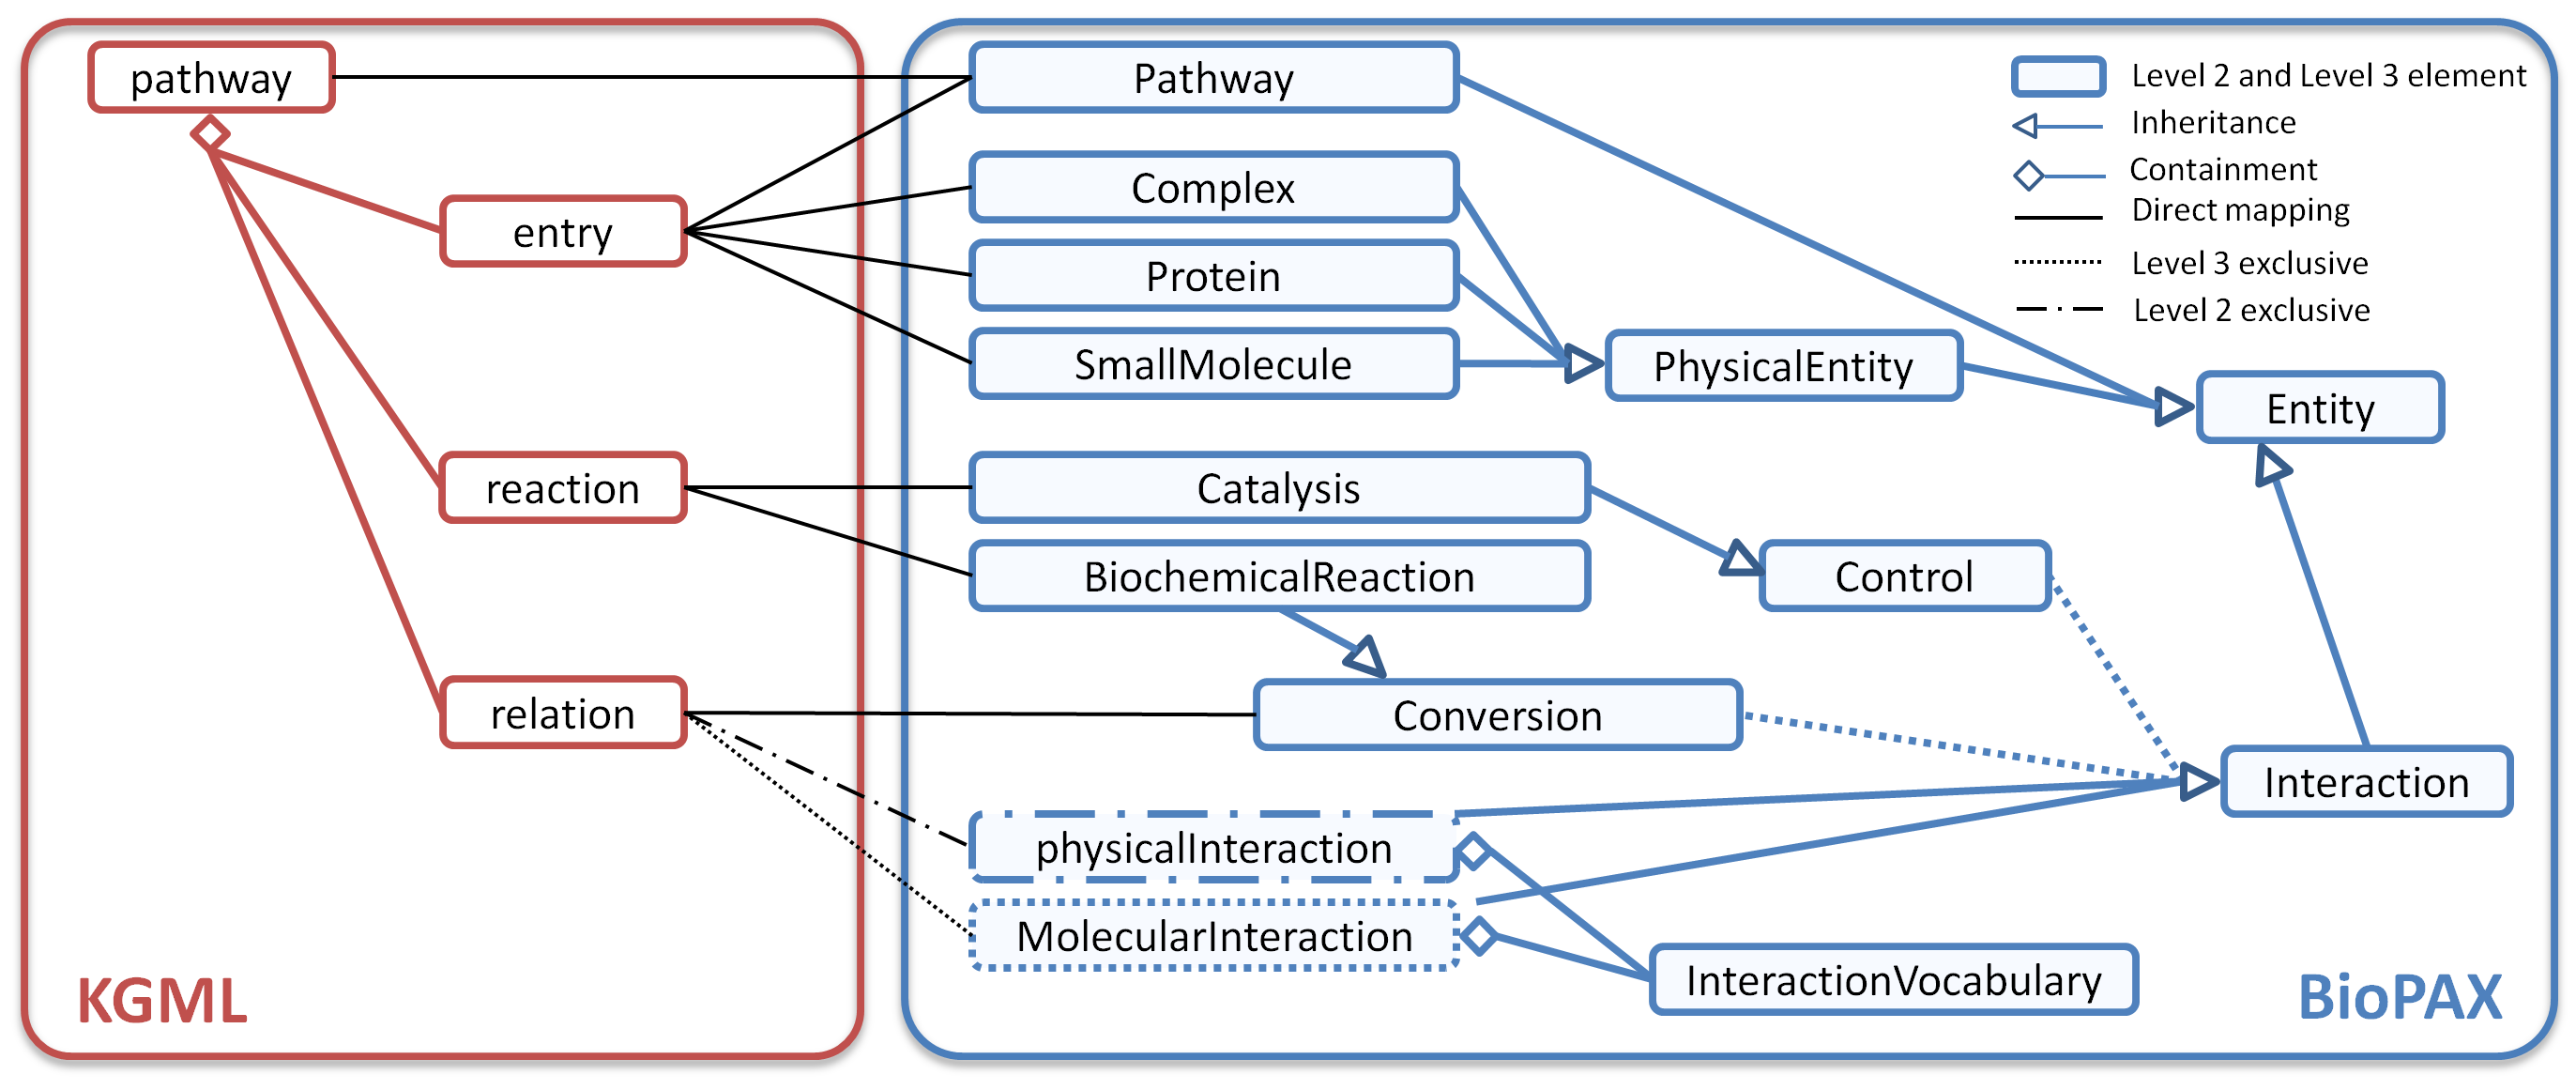
\includegraphics[width=1.0\columnwidth]{figures/KGML2BioPAX.png}
\caption{Class structure and mapping from KGML to BioPAX -- The figure shows the raw mapping of KGML to BioPAX class instances. The type attribute determines how each entry is translated (see Table~\ref{tab:KGMLentries2X}). Reactions that are catalyzed by enzymes are translated to \Catalysis{}, whereas non-catalyzed reactions are translated directly to \BiochemicalReactions. Relations are either translated to \Conversion{} or to \physicalInteraction{} in BioPAX Level 2 and \MolecularInteraction{} in Level 3 (see Table~\ref{tab:KGMLrelations2X}). To keep the clarity, the figure does not include the information that in BioPAX Level 2, \control{} and \conversion{} inherit from \physicalInteraction{}.
%Furthermore, a catalysis object contains another object that is controlled by the catalysis, which is for our purposes always a BiochemicalReaction.
Furthermore, a \Catalysis{} consists of two elements: a \Controller{} and a \Controlled{} element. For our purposes, \Controller{} is always an enzyme and \Controlled{} is a \BiochemicalReaction.
}
\label{fig:KGML2BioPAX}
\end{figure}
%%%%%%%%%%%%%%%%%%%%%%%%%%%% END FIGURE  %%%%%%%%%%%%%%%%%%%%%%%%%%%%%%%%%%%%%%%%%%%%%%%

%The preprocessed KGML document can now be translated into a BioPAX models.
Paxtools, a Java\texttrademark{} library for working with BioPAX, provides the infrastructure for building and writing the internal BioPAX data structure (\url{http://www.biopax.org/paxtools.php}). Today, BioPAX Level 2 and Level 3 are still common and there are some data structures in Level 3 that are not available in Level 2. Therefore, separate converters for BioPAX Level 2 and for Level 3 are required. First of all, a BioPAX model has to be created and a pathway object, corresponding to the input KGML, needs to be added to the model. Then, several annotations and cross-references are defined for this pathway. This includes, for instance, the organism, cross-references to other databases and gene ontology terms to define the pathway�s function. The next steps involves mapping each KGML element to a corresponding BioPAX element. Figure~\ref{fig:KGML2BioPAX} gives an overview of these mappings.

Having the initial pathway model, the next step is to create BioPAX elements for each KGML entry. This translation mainly depends on the type of the KGML entry and is listed in detail in Table~\ref{tab:KGMLentries2X}. Entries with the same identifier (graphical copies of the same element) are grouped to one instance and only one BioPAX element is created for those. Depending on the just created BioPAX element, further annotation steps are required. For \Complex'es, we need to add all components. For \SmallMolecules, we add the molecular weight and chemical formula to the corresponding BioPAX fields, which facilitates further modeling steps. For each element, cross-references to other databases and more annotations, as described in the previous section, are added.

KEGG reactions always correspond to biochemical reactions. Thus, a \BiochemicalReaction{} is the appropriate data structure for those reactions and one instance of this class is created for each reaction. If catalyzing enzymes are annotated, a \Catalysis{} instance is created. This \Catalysis{} has all catalyzing enzymes as \Controllers{} and the \BiochemicalReaction{} as \Controlled{} element. The reaction is annotated with the reaction direction and if it is reversible or not. Further, the stoichiometry of each participant is annotated, as well as the EC numbers of all catalyzing enzymes. Even to those reactions, human readable supporting information is added, like the reaction equation, other pathways in which this reaction also occurs and a generic description. In addition, the result of the atom balance check is added as further comment, together with comprehensive information which atoms are on the substrate side, which are on the product side and the difference between them.

%BioPAX not only supports biochemical reactions but also many other different types of interactions. This is especially useful to express KEGG relations, which have no associated chemical equations, but structural information like ``A activates B". These interactions include classes, for which one can specify a source and a target (useful, e.g., to express ``A inhibits B") but also interactions that just have a pool of components. The later is especially useful for cases in which information is missing or no direction is available.
Next to biochemical reactions, BioPAX also supports other kinds of relationships between entities.
BioPAX distinguishes between interactions, for which one can specify a source and a target (called \Conversion), and interactions describing a pool of interacting components (called \Interaction).
For instance, to express KEGG relations, which have no associated chemical equation but structural information like ``A activates B", a \Conversion{} can be used.
In contrast, a \Interaction{} is especially useful for cases in which information is missing or no direction is available.
%
For example, a relation of type binding with two participants -- this just allows to express ``A binds B", but no other conclusion can be drawn from such a relation. Therefore, all relations, from which no direction can be inferred, are converted to a \physicalInteraction{} in BioPAX Level 2 or to a \MolecularInteraction{} in BioPAX Level 3 (the Level 2 \physicalInteraction{} has been replaced by \MolecularInteraction{} in Level 3). All relations from which a direction can be inferred are converted to a BioPAX \Conversion{}.
An \InteractionVocabulary{} is created for each interaction, that specifies the type of interaction as SBO-term, GO-term and human-readable string. Table~\ref{tab:KGMLrelations2X} shows in detail how each relation is converted and which SBO and GO terms are being used.


\subsection{KEGG to SBML}

%%%%%%%%%%%%%%%%%%%%%%%%%%%% BEGIN FIGURE %%%%%%%%%%%%%%%%%%%%%%%%%%%%%%%%%%%%%%%%%%%%%
\begin{figure}[tb]
\centering 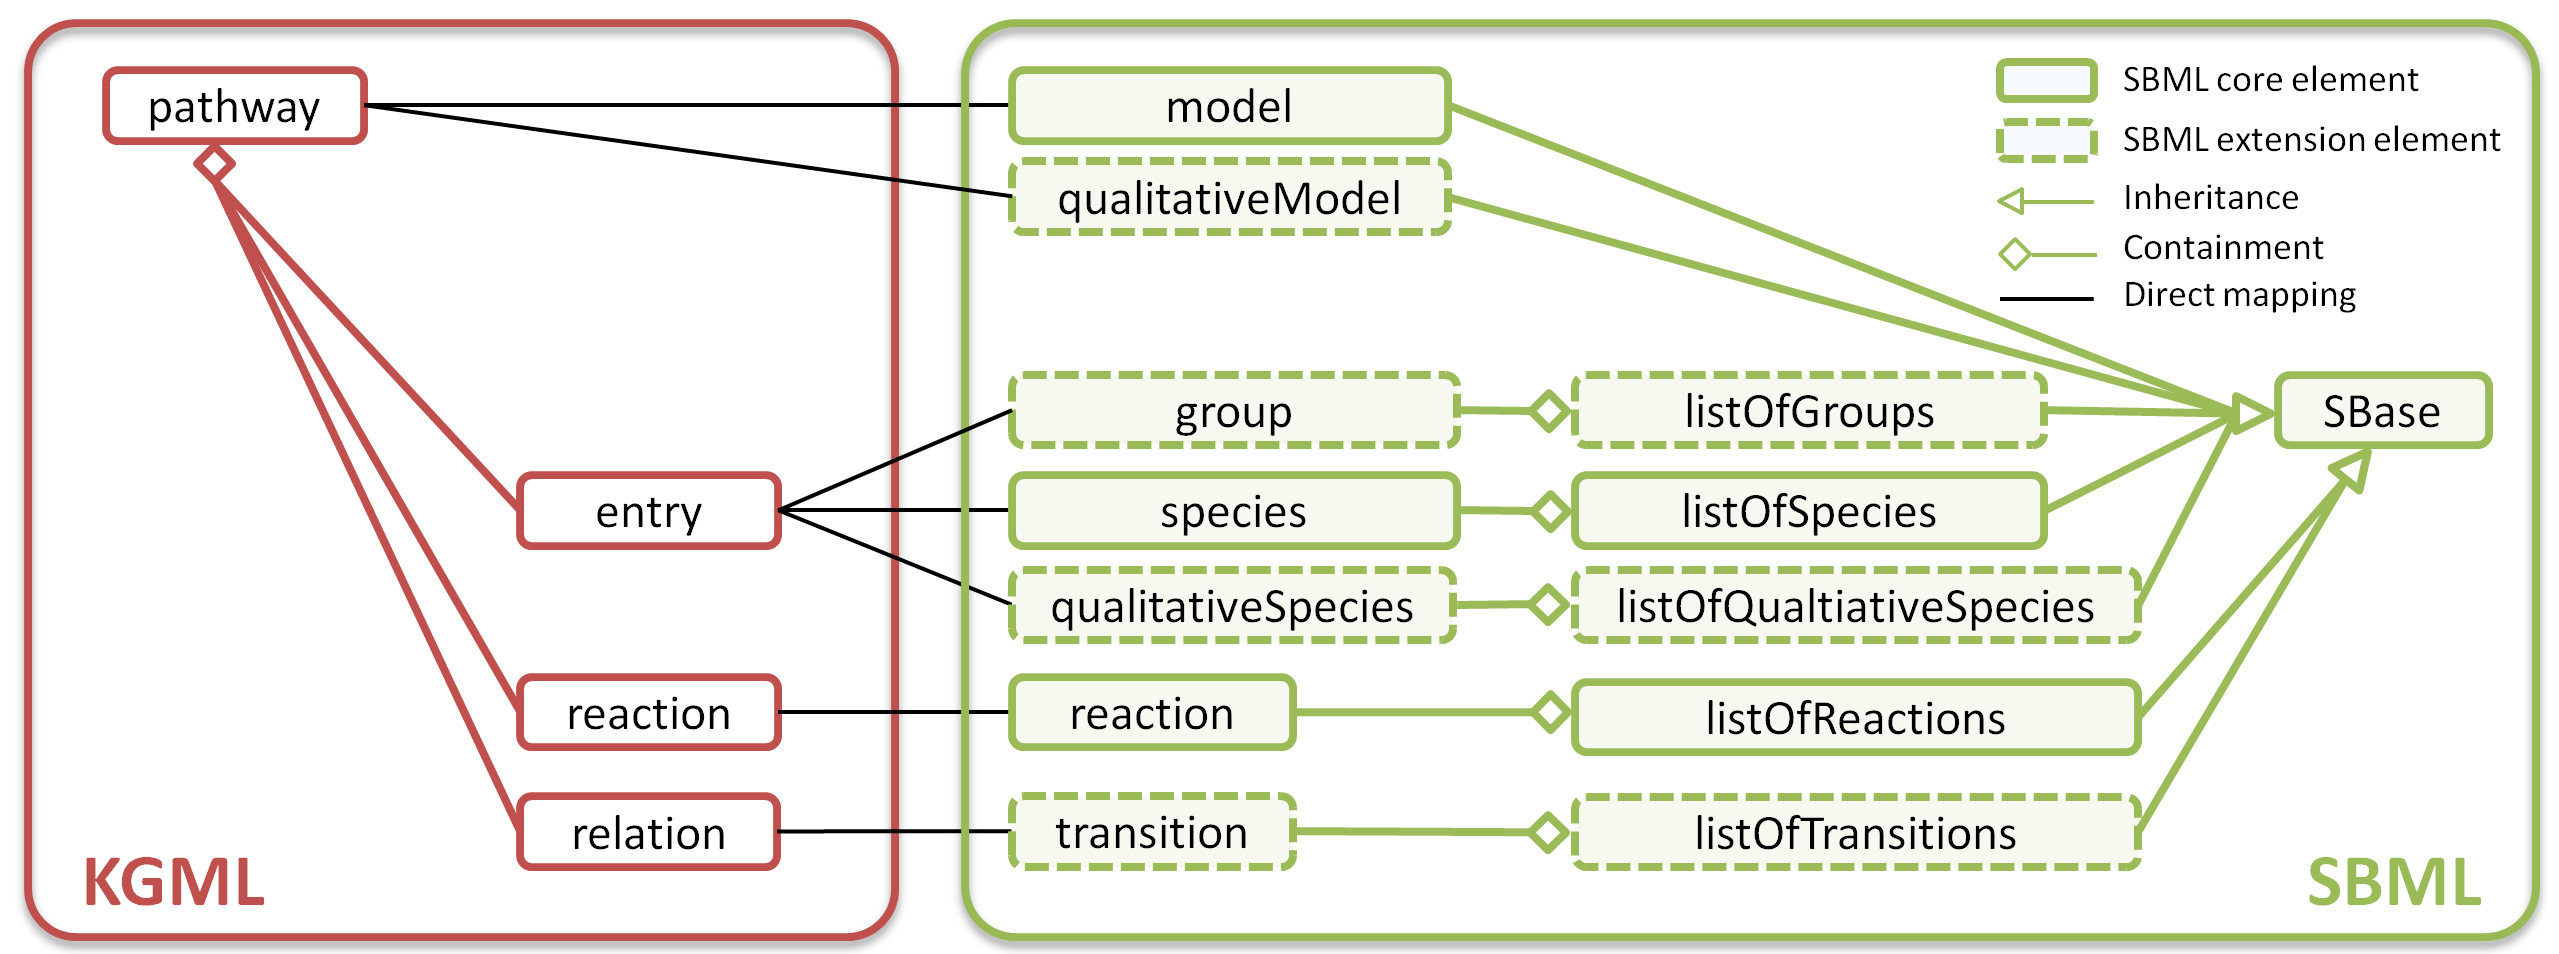
\includegraphics[width=1.0\columnwidth]{figures/KGML2SBML.png}
\caption{Class structure and mapping from KGML to SBML -- This mapping includes the SBML-qual extension package and is depicted in a simplified scheme. Most properties are encoded as attributes on the actual classes. Tables~\ref{tab:KGMLentries2X} and~\ref{tab:KGMLrelations2X} give further details about translation of entries and relations. SBML can only handle reactions, therefore SBML-qual is required to properly encode relations. This extension package requires its own model. Subsequently, the SBML-core \model{} and each \species{} have to be duplicated to obtain a \qualitativeModel{} including the translated relations.}
\label{fig:KGML2BioPAX}
\label{fig:KGML2SBML}
\end{figure}
%%%%%%%%%%%%%%%%%%%%%%%%%%%% END FIGURE %%%%%%%%%%%%%%%%%%%%%%%%%%%%%%%%%%%%%%%%%%%%%%%

% DONE: SBO-terms kodieren den typ
% keine relations => SMBL-qual
% OPTIONAL Layout extension
% DONE: Level 2/4; Level 3/1
% reactions -- reversible or irreversible, Stoichiometry, enzymes as modifiers

% EntryType reaction is skipped for core; only available for qual.

% BiologicalQualifierType, Is/HasVersion

%% QUAL:
% relations as transitions

% Viele zus�tzliche infos von kegg api
% MIRIAM identifiers
% ...including GO
% Very helpful Human readable annotations such as gene symobls, descriptions, pictures for compounds, Links to Kegg db entry, etc.

To establish the SBML data structure, we use Java\texttrademark{} library JSBML\cite{JSBML} and support SBML Level 2 Version 4\cite{SBMLl2} and SBML Level 3 Version 1\cite{SBMLl3}. The Level 3 release introduces extension packages and is required to include qualitative models (qual), groups or layout information in the document.
%
At the first glance, conversion of KGML to SBML is simple. This is also suggested by the mapping scheme, depicted in Figure~\ref{fig:KGML2SBML}. But many properties in SBML are encoded in other fields, than actual class instances and thus, are not directly visible to researchers. KEGG defines entries and an entry type, which specifies if the entry corresponds to proteins, complexes, small molecules, other pathway maps, etc. BioPAX provides different classes to distinguish between those types. SBML, similar to KGML, just has a class named \species{} to encode all those entries. The type of the \species{} should be specified by using terms from the systems biology ontology (SBO terms) \cite{SBO}. These SBO terms are hierarchically organized and only SBO terms from the ``material entity" branch should be used to encode the entities. Table~\ref{tab:KGMLentries2X} shows, which SBO terms are most appropriate to encode the different KGML entries. Furthermore, as in BioPAX translations, it is important to group graphical copies of the same entries to one element and to create only one \species{} for this entry.
To make the model usable for further applications, extensive annotations and references to other databases are added, using standardized controlled vocabulary (CV) terms and MIRIAM identifiers \cite{Juty2012,Novere2005}. Further, a description, various synonyms, the CAS number, chemical formula, reference picture (chemical image for compounds, pathway-map image for pathways), molecular weight, and mass are added as human-readable annotation, if available.

Groups are not supported by SBML. In order to encode entries of type ``group" in SBML Level 3, one can use the groups extension package \cite{SBMLgroups}. To encode groups in SBML prior to Level 3, the only way are annotations, for example by adding a CV term with a \texttt{BQB\_IS\_ENCODED\_BY} or \texttt{BQB\_HAS\_PART} qualifier, that specifies the contents of the group. In any case, an SBO-term should also be used, which defines this \species{} as a complex of multiple other \species{}.

KEGG reactions are converted to SBML \reactions{} with correct SBO terms for substrates and products. If the reaction is irreversible, different SBO terms for substrates and products should be applied. If it is reversible one should give all participating reaction components the same SBO term, e.g., SBO:0000010 (reactant). In addition, the reversibility is annotated to the \reaction{} itself and the stoichiometry is annotated on all reaction participants. Catalyzing enzymes are included as \ModifierSpeciesReference{} and CV terms, referring to the KEGG reaction identifier and all pathways, in which this reaction occurs, are added. Human-readable annotations on \reactions{} include the reaction definition, equation, a reference to the reaction equation as HTML-image, and the result of the atom balance check (i.e., if there are missing atoms in the reaction).

Relations in KEGG cannot be directly encoded in SBML. There is no structure that allows to say ``A phosphorylates B" -- we can only add whole reactions to SBML. For SBML Level 3, the recently proposed qualitative models (qual) extension package solves this problem \cite{QualSpecification}. This extension is designed for qualitative modeling and allows to
model relationships between \species{} that cannot be described in detail.
%create transitions, that just specify input, output and a relation between those.
Thus, to encode the KEGG relations, we have to convert the \model{} to a \qualitativeModel{} and create a \transition{} for each relation. An SBO term, as given in Table~\ref{tab:KGMLrelations2X}, is assigned to the \transition{} to specify the type of transition and the GO-term, mentioned in the same table, is further added as CV term on the \transition{}.




% TODO: Im Artikel auf standards pochen. Deshalb miriam, sbo, alle extensions, etc.

% Species hinzuf�gen, [ReactionModifiers merken],
% - Complex as human-readable annotation + Miriam BQB, BQB_IS_ENCODED_BY identifier.
% - SBO
% - MIRIAM (databases + reactions, description, synonyms, cas number, chemical formula, picture (for sm and pw), molecular weight, mass



%DANN Reaktionen (auch hier einmalig und eine pro id mit allen enzymen).
% -reversible
% -stoichiometry
% -SBO's hier 15=Substrate, 10=Reactant 11=Product, h�ngt von reversibility ab
% -enzyme als ModifierSpeciesReference
% Annotationen: KEGG reaction and pathway IDs
% Definition, Equation, "picture", all pws
% Check atom balance <= ADD ALSO TO BIOPAX TEXT -- result: could not check, all ok, left-right-difference

%DANN optional layout, SBGN reaction knoten auf enzym stelle, anosnten alle knoten.



%%%%%%%%%%%%%%%%%%%%%%%% RELATION TABLE %%%%%%%%%%%%%%%%%%%%%%%%
\setlength{\tabcolsep}{8pt}
\begin{sidewaystable}[p]
%\begin{table}[htbp]
%\centering
\caption{BioPAX instances and SBO terms corresponding to KGML relation subtypes}
\label{tab:KGMLrelations2X}
\makebox[\textwidth]{
%\rowcolors{1}{white}{tableShade2}
\begin{tabular}{llllll}
\toprule
KGML relation subtype           & BioPAX element & SBO term & SBO name & GO term & GO name\\
\midrule
%\multicolumn{2}{c}{\centering \textbf{BioPAX Level~2}}\\
%\midrule
%compound
%hidden compound
\rowcolor{tableShade2}
activation & conversion & SBO:0000170  & stimulation & \emph{none} & \\
inhibition & conversion & SBO:0000169  & inhibition & \emph{none} & \\
\rowcolor{tableShade2}
expression & conversion & SBO:0000170  & stimulation & GO:0010467  & gene expression \\
repression & conversion & SBO:0000169  & inhibition & \emph{none} &\\
\rowcolor{tableShade2}
indirect effect & conversion & SBO:0000344  & molecular interaction & \emph{none} & \\
state change & conversion & SBO:0000168  & control & \emph{none} & \\

\rowcolor{tableShade2}
 & physicalInteraction/ &  & & & \\
\rowcolor{tableShade2}
\multirow{-2}{*}{binding/association} &  MolecularInteraction & \multirow{-2}{*}{SBO:0000177} & \multirow{-2}{*}{non-covalent binding} & \multirow{-2}{*}{GO:0005488} & \multirow{-2}{*}{non-covalent binding} \\

 & physicalInteraction/ & &  & \\
\multirow{-2}{*}{dissociation} &  MolecularInteraction &  \multirow{-2}{*}{SBO:0000180} & \multirow{-2}{*}{dissociation} & \multirow{-2}{*}{\emph{none}} &\\

\rowcolor{tableShade2}
 & physicalInteraction/ &  & & & \\
\rowcolor{tableShade2}
\multirow{-2}{*}{missing interaction} &  MolecularInteraction & \multirow{-2}{*}{SBO:0000396} & \multirow{-2}{*}{uncertain process} &  \multirow{-2}{*}{\emph{none}} & \\

phosphorylation & conversion & SBO:0000216  & phosphorylation & GO:0016310  & phosphorylation \\
\rowcolor{tableShade2}
dephosphorylation & conversion & SBO:0000330  & dephosphorylation & GO:0016311  & dephosphorylation \\
glycosylation & conversion & SBO:0000217  & glycosylation & GO:0070085  & glycosylation \\
\rowcolor{tableShade2}
ubiquitination & conversion & SBO:0000224  & ubiquitination & GO:0016567  & ubiquitination \\
methylation & conversion & SBO:0000214  & methylation & GO:0032259  & methylation \\
%%%%%%%%%%%%%%%% TABELLE FUER 2-ZEILIG HOCHKANT %%%%%%%%%%%%%%%%
%%%%%%%%%%%%%%%%%%%%%%%%%%%%%%%%%%%%%%%%%%%%%%%%%%%%%%%%%%%%%%%%
%\multirow{2}{*}{activation} & \multirow{2}{*}{conversion} & SBO:0000170 & \emph{none} \\
% & & (stimulation)  & \\
%\multirow{2}{*}{inhibition} & \multirow{2}{*}{conversion} & SBO:0000169 & \emph{none} \\
% & & (inhibition)  & \\
%\multirow{2}{*}{expression} & \multirow{2}{*}{conversion} & SBO:0000170 & GO:0010467 \\
% & & (stimulation) & (gene expression) \\
%\multirow{2}{*}{repression} & \multirow{2}{*}{conversion} & SBO:0000169 & \emph{none} \\
% & & (inhibition) & \\
%\multirow{2}{*}{indirect effect} & \multirow{2}{*}{conversion} & SBO:0000344 & \emph{none} \\
% & & (molecular interaction)  & \\
%\multirow{2}{*}{state change} & \multirow{2}{*}{conversion} & SBO:0000168 & \emph{none} \\
% & & (control) & \\
%\multirow{2}{*}{binding/association} & physicalInteraction/ & SBO:0000177 & GO:0005488  \\
% &  MolecularInteraction & (non-covalent binding) & (non-covalent binding) \\
%\multirow{2}{*}{dissociation} & physicalInteraction/ & SBO:0000180 & \multirow{2}{*}{\emph{none}} \\
% &  MolecularInteraction & (dissociation) &  \\
%\multirow{2}{*}{missing interaction} & physicalInteraction/ &SBO:0000396 & \multirow{2}{*}{\emph{none}} \\
% &  MolecularInteraction & (uncertain process) &  \\
%\multirow{2}{*}{phosphorylation} & \multirow{2}{*}{conversion} & SBO:0000216 & GO:0016310 \\
% & & (phosphorylation) & (phosphorylation) \\
%\multirow{2}{*}{dephosphorylation} & \multirow{2}{*}{conversion} & SBO:0000330 & GO:0016311 \\
% & & (dephosphorylation) & (dephosphorylation) \\
%\multirow{2}{*}{glycosylation} & \multirow{2}{*}{conversion} & SBO:0000217 & GO:0070085 \\
% & & (glycosylation) & (glycosylation) \\
%\multirow{2}{*}{ubiquitination} & \multirow{2}{*}{conversion} & SBO:0000224 & GO:0016567 \\
% & & (ubiquitination) & (ubiquitination) \\
%\multirow{2}{*}{methylation} & \multirow{2}{*}{conversion} & SBO:0000214 & GO:0032259 \\
% & & (methylation) & (methylation) \\
%%%%%%%%%%%%%%%%%%%%%%%%%%%%%%%%%%%%%%%%%%%%%%%%%%%%%%%%%%%%%%%%
%%%%%%%%%%%%%%%%%%%%%%%%%%%%%%%%%%%%%%%%%%%%%%%%%%%%%%%%%%%%%%%%

\bottomrule
\end{tabular}
}
{

This table shows, how relations are handled during conversion to BioPAX or SBML. The conversion depends on the subtype of each relation. For each subtype, the corresponding BioPAX element as well as SBO terms and GO terms are given. When converting to BioPAX, both terms are annotated as an instance of \InteractionVocabulary, whereas an SBML \transition has a direct field for the SBO term and both terms are additionally added as CV term on the \transition.
Please note that \physicalInteraction{} in BioPAX level 2 corresponds to \MolecularInteraction{} in BioPAX level 3. Furthermore, relations of type ``compound" are treated separately, as described in a separate section of this publication.

%Erkl�ren:
%- l2 physicalInteraction, L3 MolecularInteraction
%- stets werden sbo & go verwendet, in biopax i.vocabulary mit beiden terms, in SBML der term direkt auf transition + beide als cv term.
% - compound relations

}
%\end{table}
\end{sidewaystable}
%%%%%%%%%%%%%%%%%%%%%%%%%%%%%%%%%%%%%%%%%%%%%%%%%%%%%%%%%%%%%%%%


\subsection{More KGML characteristics}

\subsubsection{KGML entries that are reactions.}
The KGML specification allows entries to have a type called ``reaction". This is used by KEGG, whenever some relation should point to a reaction, because KGML only allows entries to be targets of relations. However, BioPAX allows interactions to have no physical entities, but other interactions as sources or targets. Therefore, those entries with type ``reaction" are converted to real reactions in BioPAX and every use of this entry is replaced by using the BioPAX reaction.

In SBML, these entries are also converted to real reactions. No \species{} is created for entries with type ``reaction" in SBML-core. For SBML-qual, the specification has similar requirements as KGML: All \transitions{} must have \qualitativeSpecies{} as sources or targets. Therefore, for SBML-qual the translation is similar to the source KGML and a \qualitativeSpecies{} is created for entries with type ``reaction".

\subsubsection{Relations of subtype ``compound".}
Some KGML documents include reactions and exclusively relations of subtype ``compound". These compound-relations are mostly relations between enzymes and compounds and KEGG states that this compound is ``shared with two successive reactions [\dots]" \cite{KGML}. In other words, these relations are copies of reactions that have been created by KEGG for better graphical visualizations of the pathway. Thus, if a translation translates both, the reactions and the relations, those compound-relations contain no additional information and should be skipped.

\subsubsection{Documents with glycans instead of compounds.}
Sometimes, KGML specifies glycans as reaction participants instead of compounds. Actually, there is nothing wrong with this, except that the KEGG API often returns reaction equations with compound identifiers and attributes such as chemical formula or molecular weight are exclusively available for compounds. This leads to reactions that are erroneously detected as incorrect or to missing chemical formulas. Therefore, if a synonymous compound identifier is available for a KEGG glycan or another KEGG database identifier that contains synonyms in KEGG COMPOUND, it is advisable to fetch and internally work with the compound identifier. Else, it is very likely that duplicates of the same entries but with different identifiers are created in a model and some relationships are not correctly resolved.


%\subsection{Graphical representations}
%2GraphML (GML), 2SBGN, auch bei 2SBML wird eine visualisierung erzeugt.



%% TODO: Abgrenzung zu KEGGtranslator v1 und anderen 2BioPAX tools (related KEGG2 xy work)!



%\section{Results}
%What have we found out?
%
%Only representative results, essential for the Discussion,
%    should be presented
%Add supplementary materials for data of secondary
%    importance
%Do not attempt to "hide" data in the hope of saving it for a
%    later paper.



%\section{Discussion}
% TODO: Auf KGML eingehen
% -entries / entryType relation, genes, etc.
% -erkl�ren was reactions und relations sind
% warum nicht nur reactions/ realtions, was in welchem format, etc.
% format eigenschaften erkl�ren (SBO terms in SBML; mol.weight, chemical foruma in BioPAX
% warum initiale models, warum fix n�tig, etc.

% SBML/qual


\section{Implementation and availability of the method}
All described methods are implemented in the second release of KEGGtranslator (since version 2.0). KEGGtranslator is implemented in Java\texttrademark, provides a user-friendly and easy-to-use graphical user interface (GUI), and is freely available from \url{http://www.cogsys.cs.uni-tuebingen.de/software/KEGGtranslator/}. KGML pathways can be downloaded automatically from within KEGGtranslator. The application can convert KEGG pathways from KGML files to BioPAX Level~2, BioPAX Level~3, SBML (core), SBML (qual), or SBML-core and -qual. Furthermore, many options are provided that control the described (pre-) processing of KEGG conversions and allow for customization.

\section{Conclusion}

KEGG pathways are a valuable resource for pathway-based modeling approaches. Unfortunately, the KGML-formatted pathways are primarily for visualization purposes and not directly usable as metabolic models. Therefore, many aspects have to be fixed and considered when converting the pathways to community standards like BioPAX or SBML. This ranges from unbundling, fixing and annotating the stoichiometry on reactions, over using exclusively organism-specific and unique entities, to handling relations. Previous SBML converters have been released prior to SBML Level~3 and thus, could not include SBML extension packages \cite{KEGGconverter,KEGG2SBML}. But correctly translating relations or creating groups is not possible without the recently introduced qual \cite{QualSpecification} or groups \cite{SBMLgroups} extensions and thus, previous converters either had to skip those or create pseudo-\reactions{} or pseudo-\species{}. Until now, conversions from KEGG to BioPAX seem to be uncommon and thus, we could not find other publications or software to that we can compare our results.

We here propose methods and summarize important aspects about KEGG pathways, which can be used to create initial structural metabolic and non-metabolic models in SBML or BioPAX. All proposed methods are implemented in the KEGGtranslator application \cite{Wrzodek2011}. The models, generated by KEGGtranslator, lay the foundations for further modelling approaches, e.g., constraint-based models, tissue-specific models, or simply including kinetics to the models. All conversions obey the special requirements of SBML/BioPAX and include a huge amount of machine- and human-readable annotations. This facilitates the use of those models in other applications that perform further analysis, modeling or simulation steps on those.


\section*{Acknowledgements}
\paragraph{Funding:}
Federal Ministry of Education and Research (BMBF, Germany) in the projects Virtual Liver, Spher4Sys and the National Genome Research Network (NGFN+) under grant numbers 0315756, 0315384C and 01GS08134.

%{\TODO{Was sollten wir hier nennen ? Parkinson? Spher4Sys? Viruelle Leber? oder doch MARCAR (ich denke, das passt hier am schlechtesten)?}}

\paragraph{Conflict of interest:} None declared.

%\bibliographystyle{natbib}
\bibliographystyle{splncs}

\bibliography{KEGGtranslator_v2_methods}

\end{document} 